\section{Test di Sistema}

	\subsection{Specifica}
		I Test di Sistema hanno l'obiettivo di testare particolari proprietà globali. In particolare:
		\begin{enumerate}
			\item{\textbf{Test delle Funzionalità}: valutazione del comportamento del sistema all'esecuzione delle diverse funzionalità;}
			\item{\textbf{Test di Sicurezza}: valutazione del livello di sicurezza del sistema;}
			\item{\textbf{Test di Usabilità}: valutazione del livello di usabilità del sistema;}
			\item{\textbf{Test di Performance}: valutazione del costo di esecuzione delle funzionalità;}
			\item{\textbf{Test di Memoria/Archiviazione}: valutazioni su quantitativi di memoria necessari alla corretta esecuzione;}
			\item{\textbf{Test di Carico}: valutazione del comportamento del sistema in condizioni di carico massimo;}
			\item{\textbf{Test di Stress}: valutazione del comportamento del sistema in condizioni di sovraccarico;}
			\item{\textbf{Test di Configurazione}: valutazione del sistema in diversi ambienti di esecuzione;}
		\end{enumerate}
		Per rispettare il livello qualitativo richiesto è necessario mantenere il valore della seguente metrica entro i limiti previsti:
		\begin{itemize}
			\item{misurazione: numero di test soddisfatti;}
			\item{valore minimo accettabile: 100\%;}
			\item{valore preferibile: 100\%.}
		\end{itemize}
	
	
	\subsection{Stato}
		
		% Grafico
		\begin{figure}[H]
			\centering
			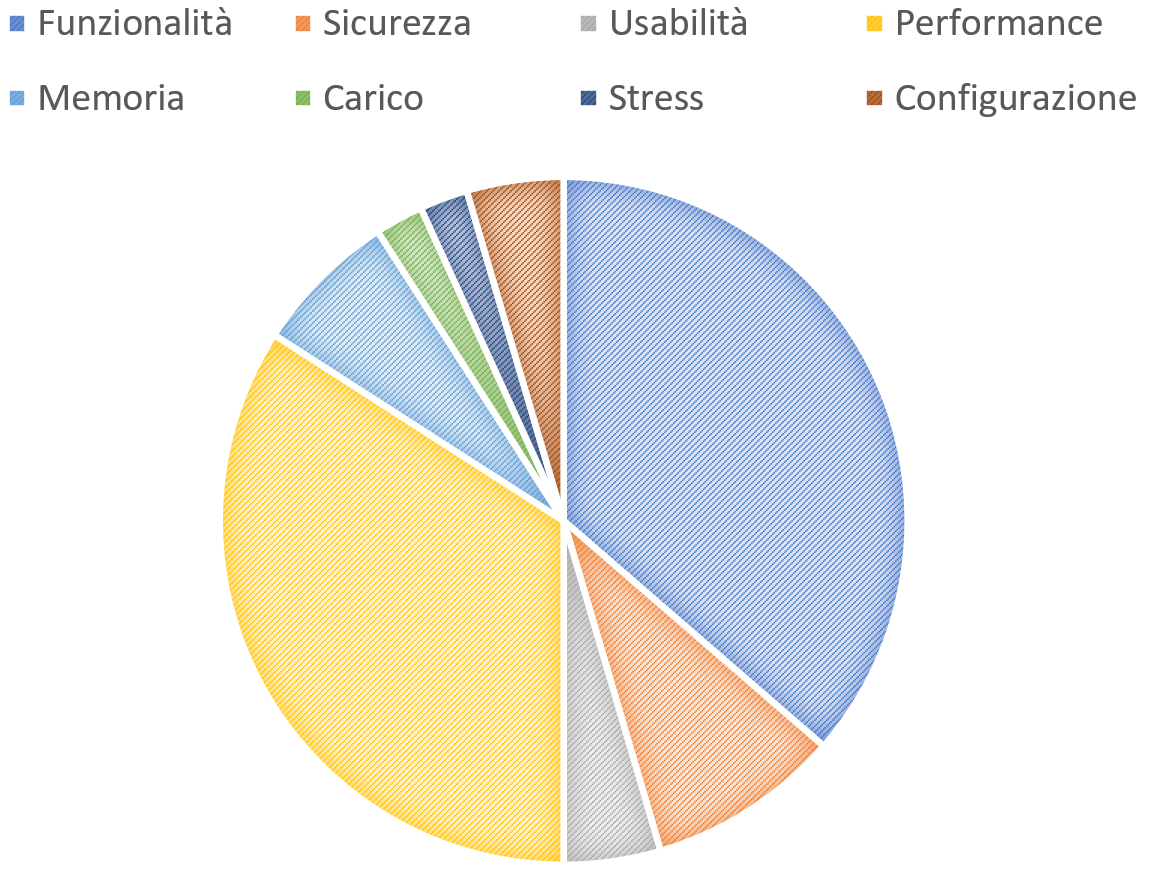
\includegraphics[width=0.6\textwidth]{./res/sections/test/sistema/graph.png}
			\caption{Suddivisione dei Test di Sistema}
		\end{figure}
	
		\def\arraystretch{1.75}
\rowcolors{2}{lightRowColor}{darkRowColor}
\begin{longtable}{
		>{\centering}p{0.12\textwidth}
		>{}p{0.5\textwidth}
		>{\centering}p{0.17\textwidth}
		>{\centering}p{0.12\textwidth} }

	\caption{Tabella dei Test di Sistema} \\
	\coloredTableHead
	\textbf{\color{white}Id Test} &
	\centering\textbf{\color{white}Descrizione} &
	\centering\textbf{\color{white}Implementato} &
	\textbf{\color{white}Superato}
	\endfirsthead

	\rowcolor{white}\caption[]{(continua)}\\
	\coloredTableHead
	\textbf{\color{white}Id Test} &
	\centering\textbf{\color{white}Descrizione} &
	\centering\textbf{\color{white}Implementato} &
	\textbf{\color{white}Superato}
	\endhead
	
	
%Funzionalità
		TF1 & Viene verificata la corretta esecuzione della funzionalità "signup". &
		Si &
		Si \tabularnewline
		
		TF2 & Viene verificata la corretta esecuzione della funzionalità "login" con private key\ped{\textit{G}}. &
		Si &
		Si \tabularnewline
		
		TF3 & Viene verificata la corretta esecuzione della funzionalità "login" con mnemonic phrase. &
		Si &
		Si \tabularnewline
		
		TF4 & Viene verificata la corretta esecuzione della funzionalità "logout". &
		Si &
		Si \tabularnewline
		
		TF5 & Viene verificata la corretta esecuzione della funzionalità "whoami". &
		Si &
		Si \tabularnewline
		
		TF6 & Viene verificata la corretta esecuzione della funzionalità "init". &
		Si &
		Si \tabularnewline
		
		TF7 & Viene verificata la corretta esecuzione della funzionalità "history". &
		Si &
		Si \tabularnewline
		
		TF8 & Viene verificata la corretta esecuzione della funzionalità "search". &
		Si &
		Si \tabularnewline
		
		TF9 & Viene verificata la corretta esecuzione della funzionalità "list" con tutte le funzioni. &
		Si &
		Si \tabularnewline
		
		TF10 & Viene verificata la corretta esecuzione della funzionalità "list" con solo le funzioni del proprietario. &
		Si &
		Si \tabularnewline
		
		TF11 & Viene verificata la corretta esecuzione della funzionalità "run". &
		Si &
		Si \tabularnewline
		
		TF12 & Viene verificata la corretta esecuzione della funzionalità "deploy\ped{\textit{G}}" senza dipendenze. &
		Si &
		Si \tabularnewline
		
		TF13 & Viene verificata la corretta esecuzione della funzionalità "deploy\ped{\textit{G}}" con dipendenze. &
		Si &
		Si \tabularnewline
		
		TF14 & Viene verificata la corretta esecuzione della funzionalità "edit" senza dipendenze. &
		Si &
		Si \tabularnewline
		
		TF15 & Viene verificata la corretta esecuzione della funzionalità "edit" con dipendenze. &
		Si &
		Si \tabularnewline
		
		TF16 & Viene verificata la corretta esecuzione della funzionalità "delete". &
		Si &
		Si \tabularnewline
		
		
		
		
%Sicurezza
		TSIC1 & Viene verificata la possibilità di eseguire la funzionalità "edit" solo su funzioni del proprietario. &
		Si &
		Si \tabularnewline
		
		TSIC2 & Viene verificata la possibilità di eseguire la funzionalità "delete" solo su funzioni del proprietario. &
		Si &
		Si \tabularnewline
		
		TSIC3 & Viene verificata l'impossibilità di ritornare le credenziali AWS\ped{\textit{G}} del sistema, tramite l'esecuzione di una funzione Lambda\ped{\textit{G}}. &
		Si &
		Si \tabularnewline
		
		TSIC4 & Viene verificata l'impossibilità di eseguire funzioni con tempo di esecuzione o richiesta risorse superiori ai limiti previsti.  &
		Si &
		Si \tabularnewline
		
		
		
		
		
		
%Usabilità
		TUS1 & Viene valutata la leggibilità dei manuali, tramite il calcolo di valori accettabili per l'indice di Flesh. &
		Si &
		Si \tabularnewline
		
		TUS2 & Viene valutato il numero di funzionalità a supporto dell'utente. &
		Si &
		Si \tabularnewline




%Performance
		TP1 & Viene valutato il costo di esecuzione della funzionalità "signup". &
		Si &
		Si \tabularnewline
		
		TP2 & Viene valutato il costo di esecuzione della funzionalità "login". &
		Si &
		Si \tabularnewline
		
		TP3 & Viene valutato il costo di esecuzione della funzionalità "logout". &
		Si &
		Si \tabularnewline
		
		TP4 & Viene valutato il costo di esecuzione della funzionalità "whoami". &
		Si &
		Si \tabularnewline
		
		TP5 & Viene valutato il costo di esecuzione della funzionalità "init". &
		Si &
		Si \tabularnewline
		
		TP6 & Viene valutato il costo di esecuzione della funzionalità "history". &
		Si &
		Si \tabularnewline
		
		TP7 & Viene valutato il costo di esecuzione della funzionalità "search". &
		Si &
		Si \tabularnewline
		
		TP8 & Viene valutato il costo di esecuzione della funzionalità "list". &
		Si &
		Si \tabularnewline
		
		TP9 & Viene valutato il costo di esecuzione della funzionalità "list" con solo le funzioni del proprietario. &
		Si &
		Si \tabularnewline
		
		TP10 & Viene valutato il costo di esecuzione della funzionalità "run". &
		Si &
		Si \tabularnewline
		
		TP11 & Viene valutato il costo di esecuzione della funzionalità "deploy\ped{\textit{G}}" senza dipendenze. &
		Si &
		Si \tabularnewline
		
		TP12 & Viene valutato il costo di esecuzione della funzionalità "deploy\ped{\textit{G}}" con dipendenze. &
		Si &
		Si \tabularnewline
		
		TP13 & Viene valutato il costo di esecuzione della funzionalità "edit" senza dipendenze. &
		Si &
		Si \tabularnewline
		
		TP14 & Viene valutato il costo di esecuzione della funzionalità "edit" con dipendenze. &
		Si &
		Si \tabularnewline
		
		TP15 & Viene valutato il costo di esecuzione della funzionalità "delete". &
		Si &
		Si \tabularnewline
		
		
		
		
		
		
		
%Memoria/Archiviazione
		TM1 & Viene valutato il quantitativo di memoria necessario all'installazione dell'applicativo. &
		Si &
		Si \tabularnewline
		
		TM2 & Viene valutato il quantitativo di memoria utilizzata da EBS per il mantenimento del server. &
		Si &
		Si \tabularnewline
		
		TM3 & Viene valutato il quantitativo di memoria utilizzata da AWS Lambda\ped{\textit{G}} per l'esecuzione di funzioni. &
		Si &
		Si \tabularnewline
		




%Test di carico
		TC1 & Viene verificato il corretto funzionamento in caso di 1000 richieste concorrenti. &
		Si &
		Si \tabularnewline
		



%Test di stress
		TSTR1 & Viene verificato il corretto funzionamento in caso di oltre 1000 richieste concorrenti. &
		Si &
		Si \tabularnewline
		
		
		
		
%Test di configurazione
		TCONF1 & Viene verificata la corretta installazione in ambiente\ped{\textit{G}} Windows. &
		Si &
		Si \tabularnewline
		
		TCONF2 & Viene verificata la corretta installazione in ambiente\ped{\textit{G}} Linux. &
		Si &
		Si \tabularnewline


\end{longtable}
